\subsection{UC2 - Visualizzazione dei dati}
\label{uc2}

    \begin{figure}[htbp]
        \centering
        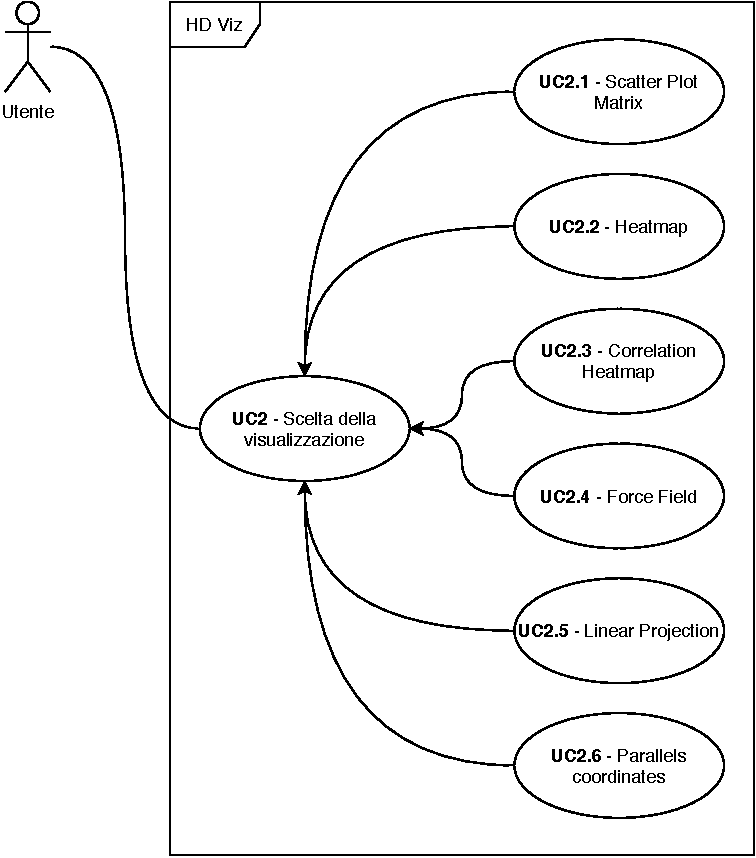
\includegraphics[width=0.7\textwidth]{source/sections/casi-uso/diagrams/uc2.pdf}
        \caption{UC2 - Visualizzazione dei dati}
        \label{fig:uc2}
    \end{figure}

    % \includegraphics{}
    \begin{itemize}
    \item \textbf{Attore}: utente;
    \item \textbf{Descrizione}: l'utente all'interno dell'applicazione visualizza i dati
    \item \textbf{Precondizione}:
    \begin{itemize}
        \item il sistema è funzionante e raggiungibile;
        \item eseguito l'upload del dataset come matrice $N\times M$ (\hyperref[uc1.1]{UC1.1});
    \end{itemize}
    \item \textbf{Postcondizione}: l'utente visualizza i dati tramite uno dei grafici disponibili
    \item \textbf{Scenario Principale}: 
        \begin{enumerate}
            \item l'utente visualizza il grafico costruito a partire dai dati caricati.
        \end{enumerate}  
    \end{itemize}
    
    \subsubsection{UC2.1 - Visualizzazione grafico}
    \label{uc2.1}
    % \includegraphics{}
    \begin{itemize}
    \item \textbf{Attore}: utente;
    \item \textbf{Descrizione}: l'utente all'interno dell'applicazione visualizza il grafico
    \item \textbf{Precondizione}:
    \begin{itemize}
        \item il sistema è funzionante e raggiungibile;
        \item eseguito l'upload del dataset come matrice $N\times M$ (\hyperref[uc1.1]{UC1.1});
    \end{itemize}
    \item \textbf{Postcondizione}: l'utente visualizza il grafico scegliendo fra un tipo di quelli disponibili
    \item \textbf{Scenario Principale}: 
        \begin{enumerate}
            \item l'utente visualizza il grafico costruito a partire dal dataset caricato.
        \end{enumerate}  
    \item \textbf{Generalizzazioni}:
        \begin{enumerate}
            \item l'utente visualizza il grafico scegliendo il tipo tra uno di quelli disponibili:
                \begin{enumerate}
                    \item Scatter Plot Matrix (\hyperref[uc2.1.1]{UC2.1.1});
                    \item Heatmap (\hyperref[uc2.1.2]{UC2.1.2});
                    \item Correlation Heatmap (\hyperref[uc2.1.3]{UC2.1.3});
                    \item Force Field (\hyperref[uc2.1.4]{UC2.1.4});
                    \item Linear Projection (\hyperref[uc2.1.5]{UC2.1.5});
                    \item Parallel Coordinates (\hyperref[uc2.1.6]{UC2.1.6}).
                \end{enumerate}
        \end{enumerate}  
    \end{itemize}
    
    %%%
    \paragraph{UC2.1.1 - Scatter Plot Matrix}
    \label{uc2.1.1}
    \begin{itemize}
    \item \textbf{Attore}: utente;
    \item \textbf{Descrizione}: l'utente visualizza il dataset caricato tramite grafico \emph{Scatter Plot Matrix};
    \item \textbf{Precondizione}:
    \begin{itemize}
        \item il sistema è funzionante e raggiungibile;
        \item eseguito l'upload del dataset come matrice $N\times M$ (\hyperref[uc1.1]{UC1.1});
        \item le features del dataset da visualizzare sono al massimo 5
    \end{itemize}
    \item \textbf{Postcondizione}: l'utente visualizza il dataset caricato tramite grafico \emph{Scatter Plot Matrix};
    \item \textbf{Scenario Principale}: 
        \begin{enumerate}
            \item l'utente visualizza il grafico \emph{Scatter Plot Matrix} ricavato dal dataset caricato.
        \end{enumerate}
    \end{itemize}
    
    %%%
    \paragraph{UC2.1.2 - Heatmap}
    \label{uc2.1.2}
    \begin{itemize}
    \item \textbf{Attore}: utente;
    \item \textbf{Descrizione}: l'utente visualizza il dataset caricato tramite grafico \emph{Heatmap};
    \item \textbf{Precondizione}:
    \begin{itemize}
        \item il sistema è funzionante e raggiungibile;
        \item eseguito l'upload del dataset come matrice $N\times M$ (\hyperref[uc1.1]{UC1.1});
    \end{itemize}
    \item \textbf{Postcondizione}: l'utente visualizza il dataset caricato tramite grafico \emph{Heatmap};
    \item \textbf{Scenario Principale}: 
        \begin{enumerate}
            \item \item l'utente visualizza il grafico \emph{Heatmap} ricavato dal dataset caricato.
        \end{enumerate}
    \end{itemize}
    
    %%%
    \paragraph{UC2.1.3 - Correlation Heatmap}
    \label{uc2.1.3}
    \begin{itemize}
    \item \textbf{Attore}: utente;
    \item \textbf{Descrizione}: l'utente visualizza il dataset caricato tramite grafico \emph{Correlation Heatmap};
    \item \textbf{Precondizione}:
    \begin{itemize}
        \item il sistema è funzionante e raggiungibile;
        \item eseguito l'upload del dataset come matrice $N\times M$ (\hyperref[uc1.1]{UC1.1});
    \end{itemize}
    \item \textbf{Postcondizione}: l'utente visualizza il dataset caricato tramite grafico \emph{Correlation Heatmap};
    \item \textbf{Scenario Principale}: 
        \begin{enumerate}
            \item l'utente visualizza il grafico \emph{Correlation Heatmap} ricavato dal dataset caricato.
        \end{enumerate}
    \end{itemize}
    
    %%%
    \paragraph{UC2.1.4 - Force Field}
    \label{uc2.1.4}
    \begin{itemize}
    \item \textbf{Attore}: utente
    \item \textbf{Descrizione}: l'utente visualizza il dataset caricato tramite grafico \emph{Force Field};
    \item \textbf{Precondizione}:
    \begin{itemize}
        \item il sistema è funzionante e raggiungibile;
       \item eseguito l'upload del dataset come matrice $N\times M$ (\hyperref[uc1.1]{UC1.1});
    \end{itemize}
    \item \textbf{Postcondizione}: l'utente visualizza il dataset caricato tramite grafico \emph{Force Field};
    \item \textbf{Scenario Principale}: 
        \begin{enumerate}
            \item l'utente visualizza il grafico \emph{Force Field} ricavato dal dataset caricato.
        \end{enumerate}
    \end{itemize}
    
    %%%
    \paragraph{UC2.1.5 - Linear Projection}
    \label{uc2.1.5}
    \begin{itemize}
    \item \textbf{Attore}: utente;
    \item \textbf{Descrizione}: l'utente visualizza il dataset caricato tramite grafico \emph{Linear Projection};
    \item \textbf{Precondizione}:
    \begin{itemize}
        \item il sistema è funzionante e raggiungibile;
        \item eseguito l'upload del dataset come matrice $N\times M$ (\hyperref[uc1.1]{UC1.1});
    \end{itemize}
    \item \textbf{Postcondizione}: l'utente visualizza il dataset caricato tramite grafico \emph{Linear Projection};
    \item \textbf{Scenario Principale}: 
        \begin{enumerate}
            \item l'utente visualizza il grafico \emph{Linear Projection} ricavato dal dataset caricato
        \end{enumerate}
    \end{itemize}
    
    %%%
    \paragraph{UC2.1.6 - Parallel Coordinates}
    \label{uc2.1.6}
    
    \begin{itemize}
    \item \textbf{Attore}: utente;
    \item \textbf{Descrizione}: l'utente visualizza il dataset caricato tramite grafico \emph{Parallel Coordinates};
    \item \textbf{Precondizione}:
    \begin{itemize}
        \item il sistema è funzionante e raggiungibile;
        \item eseguito l'upload del dataset come matrice $N\times M$ (\hyperref[uc1.1]{UC1.1});
    \end{itemize}
    \item \textbf{Postcondizione}: l'utente visualizza il dataset caricato tramite grafico \emph{Parallel Coordinates};
    \item \textbf{Scenario Principale}:
        \begin{enumerate}
            \item l'utente visualizza il grafico \emph{Parallel Coordinates} ricavato dal dataset caricato
        \end{enumerate}
    \end{itemize}
    
  
